% teleconnections chapter

\Chapter{pyleogrid}{An Ensemble method for Gridding Paleo Proxy Climates}

\label{chp:gridding}

\begin{refsection}

%----------------------------------------------------------------------------------------
%	SECTION 1
%----------------------------------------------------------------------------------------

\section{Introduction}  \label{sec:gridding-intro}

\begin{itemize}
	\item Why gridding
	\begin{itemize}
		\item Data-Model-Intercomparisons)
		\item Easier to handle
		\item Energy balance, compatibility with models, grid cell (Area) averages
		\item Stability of observation network through time
		\item Not just spatial grid, also regular timestep (problems with pseudo gridding, including time ‘windows’ or ‘slices’
		\item Understanding past climates, different forcings – independent of models (difficult from point-cloud)
		\item Filling the gaps
		\item Spatial scales (Samarthein chironomids etc)
	\end{itemize}
	\item Importance of uncertainties
	\begin{itemize}
		\item Necessary for data comparisons, interpretation skill of the data
		\item Proxy climate reconstruction uncertainties are higher (inverse modelling, not always properly defined (MAT)) than for instrumental data
		\item Age uncertainties can be high (centennial to multi-millennial)
	\end{itemize}
	\item Why Tps (can also use something else, but has been used before)
	\begin{itemize}
		\item Extrapolation to the gaps (Previous work by mauri et al and davis)
		\item Pseudo-gridding (marcott, Marsicek 2018, Margo, 2009, Bartlein et al ?2013) has holes
		\item Data assimiliation (pages2k? Need to look the paper up again) – depends on model
		\item Bayesian data assimiliation (Weitzel 2019) – depends on model
		\item Does not require interpolation of time (Marsicek 2018)
	\end{itemize}
	\item Other
	\item Introducing constraints; climate, training set size, spatial coverage etc
\end{itemize}


\section{Data}  \label{sec:gridding-data}

The ensemble based gridding method is adapted to paleo-climates. In this study, we describe the method using a large set of western Eurasian fossil pollen assemblages that have been transformed to \gls{jja} temperatures. We focus on pollen data because it is the spatially most widely available proxy during the Holocene, but it is important to mention that the reconstruction method is agnostic to the climate proxy, because it does not explicitly use the pollen assemblages but rather alters the standard climate reconstruction method under the aspect of it's methodological uncertainties. As such, the following sections describe the fossil and modern pollen database for this use case (section \ref{sec:gridding-polnet}) and the associated uncertainties of the temperature reconstruction method (section \ref{sec:gridding-mat}) and the dating of the fossil pollen samples (section \ref{sec:gridding-ageunc}).

\subsection{Pollen database}  \label{sec:gridding-polnet}

\begin{figure}
	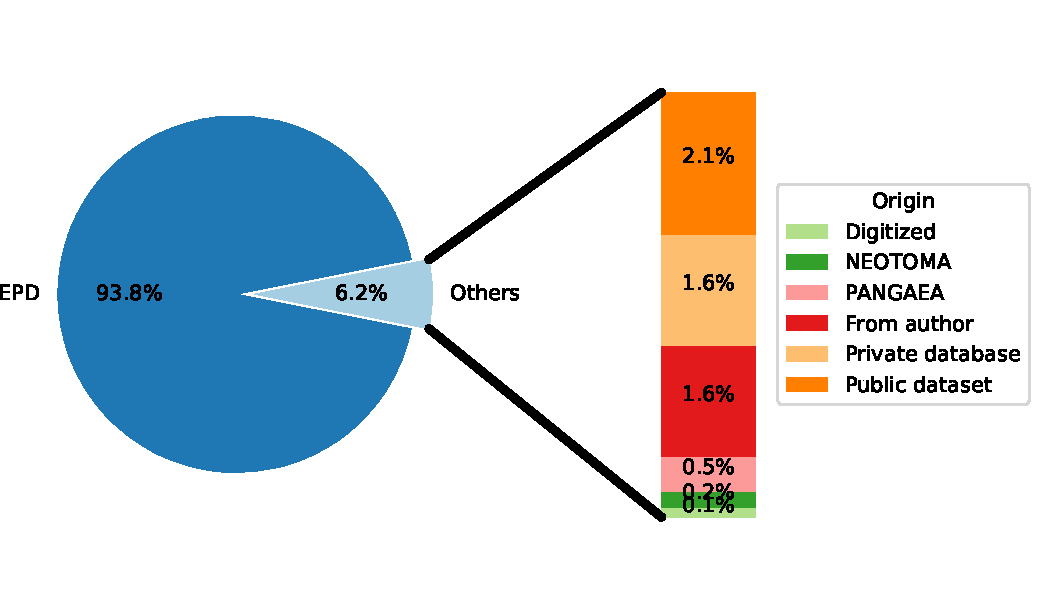
\includegraphics[width=\linewidth]{gridding-figures/origins.pdf} \\
	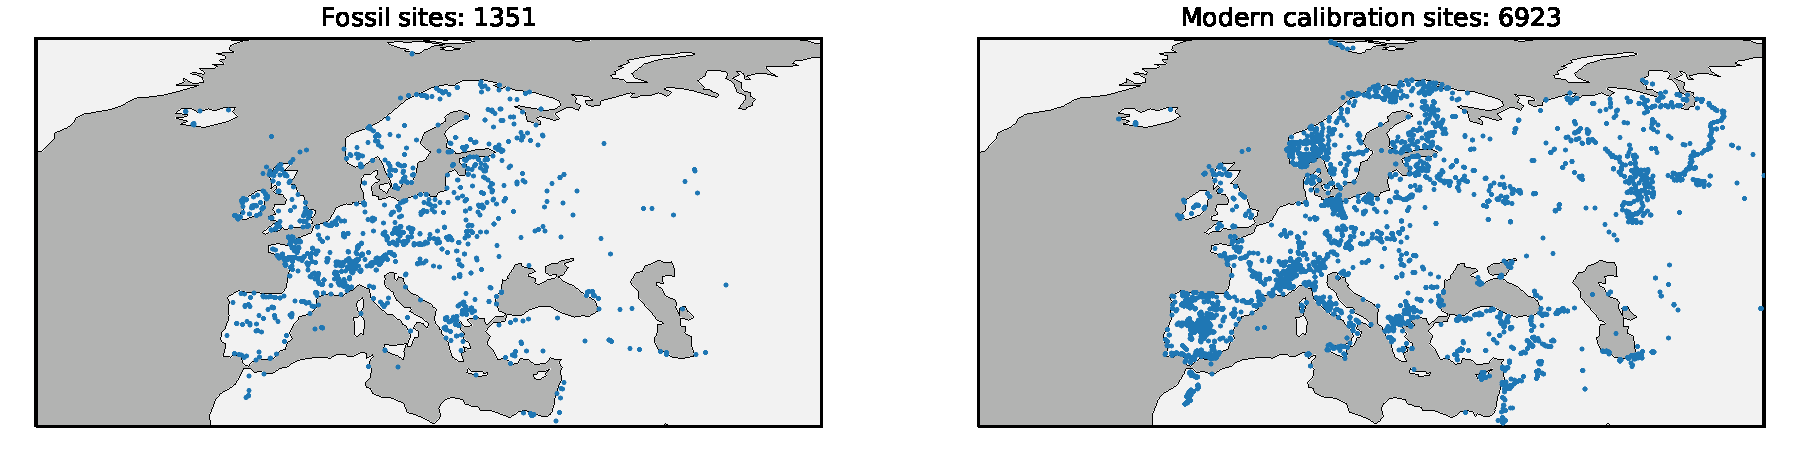
\includegraphics[width=\linewidth]{gridding-figures/sitelocs.pdf}
	\caption[Fossil Pollen Database]{Data origins for the fossil POLNET database in western Eurasia (1351 in total). The majority comes from the \gls{epd} and other public datasets, and some sites where obtained through direct communication from the authors and private databases.}
	\label{fig:gridding-fossil}
\end{figure}

The source data for this study is a subset of the latest development version of the POLNET database, a northern hemispheric, sub-tropical collection of pollen assemblages \citep{DavisKaplan2017, SommerDavisChevalierEtAl2019}. The purpose of this database is to generate the source for large-scale climate reconstruction during the Holocene (past 12'000 years) that can be used for model-data comparisons. The subset that we use in this study to describe and develop the gridding method contains fossil and modern pollen assemblages of western Eurasia, a region that has already been under investigation in the previous study by \cite{MauriDavisCollinsEtAl2015}. 

The database contains raw pollen counts from various publicly available and private data sources, in total 1350 datasets with 80500 fossil samples. The majority of the fossil pollen data (see figure \ref{fig:gridding-fossil}) comes from the \gls{epd} (94\%), other publicly available databases \addref[Binney, Cao et al., 2019, ACER database], and PANGAEA. The  rest has been obtained either through private communications from the author\addref[probably not possible...], the private database that has also been used by \cite{MauriDavisCollinsEtAl2015}, and 2 sites have been digitized.

\begin{figure}
	\missingfigure{Modern calibration data (ask Manu)}
	\caption{Modern calibration database}
	\label{fig:gridding-modern}
\end{figure}

The modern calibration dataset (XXXX samples, see figure \ref{fig:gridding-modern}) is mainly based on the version 2 of the \gls{empd} \citep{DavisZanonCollinsEtAl2013}\todo{Describe origins of modern calibration data, link back to chapter \ref{chp:empd}}. 


\subsection{Site-based holocene temperature estimates}  \label{sec:gridding-mat}
A standard approach for site-based climate reconstruction from fossil pollen assemblages is the so-called \glsfirst{mat} (also called $k$-nearest neighbors). This technique estimates the climate of the fossil sample as the (weighted) climate average of the most similar modern samples (i.e. the closest modern analogues). It has the major advantage that it requires little parameterization efforts and can be applied over a large spatial area that covers many different climate regimes \citep{MauriDavisCollinsEtAl2015}. We apply this method but vary it in our probabilistic setup, such that it better represents the spatial domain of the modern analogues.

For this purpose, we follow the standard approach and assign a \gls{jja} temperature to each modern calibration sample (figure \ref{fig:gridding-modern}), taken from the corresponding grid cell in the WorldClim dataset, version 2 at 30 seconds \citep{FickHijmans2017}.

In the next step every pollen assemblage is transformed from raw counts to percentages, based on the total sum of terrestrial pollen counts in the sample. In order to measure the similarity between a (transformed) fossil pollen assemblages $\left\lbrace f_{i}\right\rbrace$ and modern pollen assemblage $\left\lbrace m_{i}\right\rbrace$ with use squared-chord distance from the R package \textit{rioja} \citep{Juggins2017}, defined as

\begin{equation*}
d = \sum_{i}\left(\sqrt{f_{i}} - \sqrt{m_{i}}\right)^2
\end{equation*}

This is done for every modern and fossil sample in the database. The standard, non-probabilistic setup would now compute the climate of the fossil sample as the mean climate of the $k$ closest analogues (e.g. $k = 6$), eventually weighted by their corresponding distance $d$. There are many variations of this technique (see for example \cite{BirksHeiriSeppaeEtAl2010}, including various measures of similarity\addref, choices about $k$\addref, the maximum allowed distance $d$ between modern and fossil assemblage\addref, subsampling of the calibration dataset to avoid spatial autocorrelation\addref[Guiot and de Vernal, 2011; Telford and Birks, 2009, 2005], and by grouping pollen taxa into so-called plant-functional types (PFTs) \citep[e.g.]{DavisBrewerStevensonEtAl2003, MauriDavisCollinsEtAl2015}. They all, however, have in common that the categorical, multi-modal distribution of the climate of the modern analogues is oversimplified into a unimodal distribution represented by the mean of the analogue climates. Therefore, in our ensemble approach, we explicitly do not take the mean but sample the climate of the analogues directly. This is further discussed in the methods section \ref{sec:gridding-temperature-sampling} and \ref{sec:gridding-site}.


\subsection{Age uncertainties}  \label{sec:gridding-ageunc}
In addition to the methodological uncertainties of the climate reconstruction method (previous section \ref{sec:gridding-mat}), we provide a framework to handle dating uncertainties. During the gridding step (see next section \ref{sec:gridding-gridding}), every sample is weighted by the age difference to the target reconstruction age. The previous studies by \cite{DavisBrewerStevensonEtAl2003} and \cite{MauriDavisCollinsEtAl2015} do not take this uncertainty, that can be as high as multiple centuries, into account although they influence the gridded temperature reconstruction.

The reason is a systematic problem of pollen samples that we overcome here with the recent developments in the pollen community. In palynology, each sample in a sediment core is is dated using a so-called age-depth model, a function that maps each depth of the sediment core to an age. This function is based on a few chronological control points where the age has been determined instrumentally (for lake sediments in the Northern Hemisphere, these are commonly radiocarbon ($^{14}$C dates) and interpolates/extrapolates to the depths of the sample locations. Various methodologies exist to define these age-depth models, ranging from simple linear interpolation methods \citep{Bennett1994} to the more recently developed bayesian techniques of the Bchron \citep{HaslettParnell2008} and BACON \citep{BlaauwChristen2011} models.

The early approaches have been proven to provide unreliable uncertainty estimates \citep{TelfordHeegaardBirks2004} and there has been no standardized way to report the uncertainties, if they are reported at all. For this reason we (and previous studies) cannot rely on the age uncertainties reported in the pollen database. An alternative approach is to recalculate the chronology for every dataset in the database \citep[see][for instance]{Goring2019}, but this also requires parameterization for reliable uncertainties and goes beyond the scope of this study.

Instead, we follow an approach that is based on two aspects: age uncertainties are higher for older samples, and samples that are farther away from the radiocarbon dates (i.e. chronological control points). Additionally, samples behave differently if the sample is surrounded by two chronological points (i.e. the sampe age is interpolated) or not (sample age is extrapolated). These relationships are illustrated in figure \ref{fig:gridding-univariate-unc}, based on all datasets (ca. 30'000 samples) from the Neotoma paleoecology database \citep{WilliamsGrimmBloisEtAl2018} that have age-depth models estimated with BACON, a model that has been proven to provide more reliable age uncertainty estimates \citep{TrachselTelford2016}. These uncertainties in Neotoma are reported as two sigma confidence intervals of lower and upper sample age bounds, but for the sake of implementation (section \ref{sec:gridding-age-sampling} assumes a normal distribution), we use the one sigma uncertainty of the maximum of the two deviations. The grayscale density plots in the background shows the high dispersal of the data and the number of samples decreases strongly with higher distance to the control point or older samples (red lines). Nonetheless, the mean of the data (blue lines) reveals the increasing nature of both relationships, as mentioned before.

Figure \ref{fig:gridding-univariate-unc} also shows two models that have been fitted to the data. The first one is a standard simple univariate linear model $y = a + b\cdot x$ (orange line). This model already simulates the increasing trend of both variables although it does not capture the non-linear relationship between age and age-uncertainty. A possible reasons for this non-linearity might be the time-dependency of the radiocarbon calibration curve and it's associated errors. This gives the motivation to use a constrained linear \glsfirst{gam}, a smooth semi-parametric model of the form

\begin{equation*}
	\mathbb{E}[y|X] = \beta_0+f_1(X_1)
\end{equation*}

in the univariate case, or

\begin{equation*}
\mathbb{E}[y|X] = \beta_0+f_1(X_1)+f_2(X_2)
\end{equation*}

in the bivariate case. The feature functions $f_{1,2}$ are based on penalized B splines with a constraint for monotonic increasing, $\mathbb{E}[y|X]$ is based on a normal distribution and has been fitted with the \textit{pyGAM} software package \citep{ServenBrummittAbedi2018}. This model enables to better simulate the non-linear features as can be seen with the green lines in figure \ref{fig:gridding-univariate-age-unc}.

These results approve the initial hypotheses and justify the choice of a bivariate \gls{gam} for predicting age uncertainties based on the distance to the chronological control point, and the age of the sample. The two models, together with a bivariate simple linear regression model, and again for interpolated and extrapolated samples, are shown in the central column of figure \ref{fig:gridding-bivariate-age-unc}. Both model classes (simple linear and \gls{gam}) are able to reproduce the general shape of the observed data, although the \gls{gam} better resolves the non-linear relationship between the three variables.

The final uncertainties, predicted for the data set presented in the previous section \ref{sec:gridding-polnet}, are shown in the supplementary figure \ref{fig:gridding-age-uncertainties}.

\begin{figure}
	\captionsetup{width=\linewidth}
	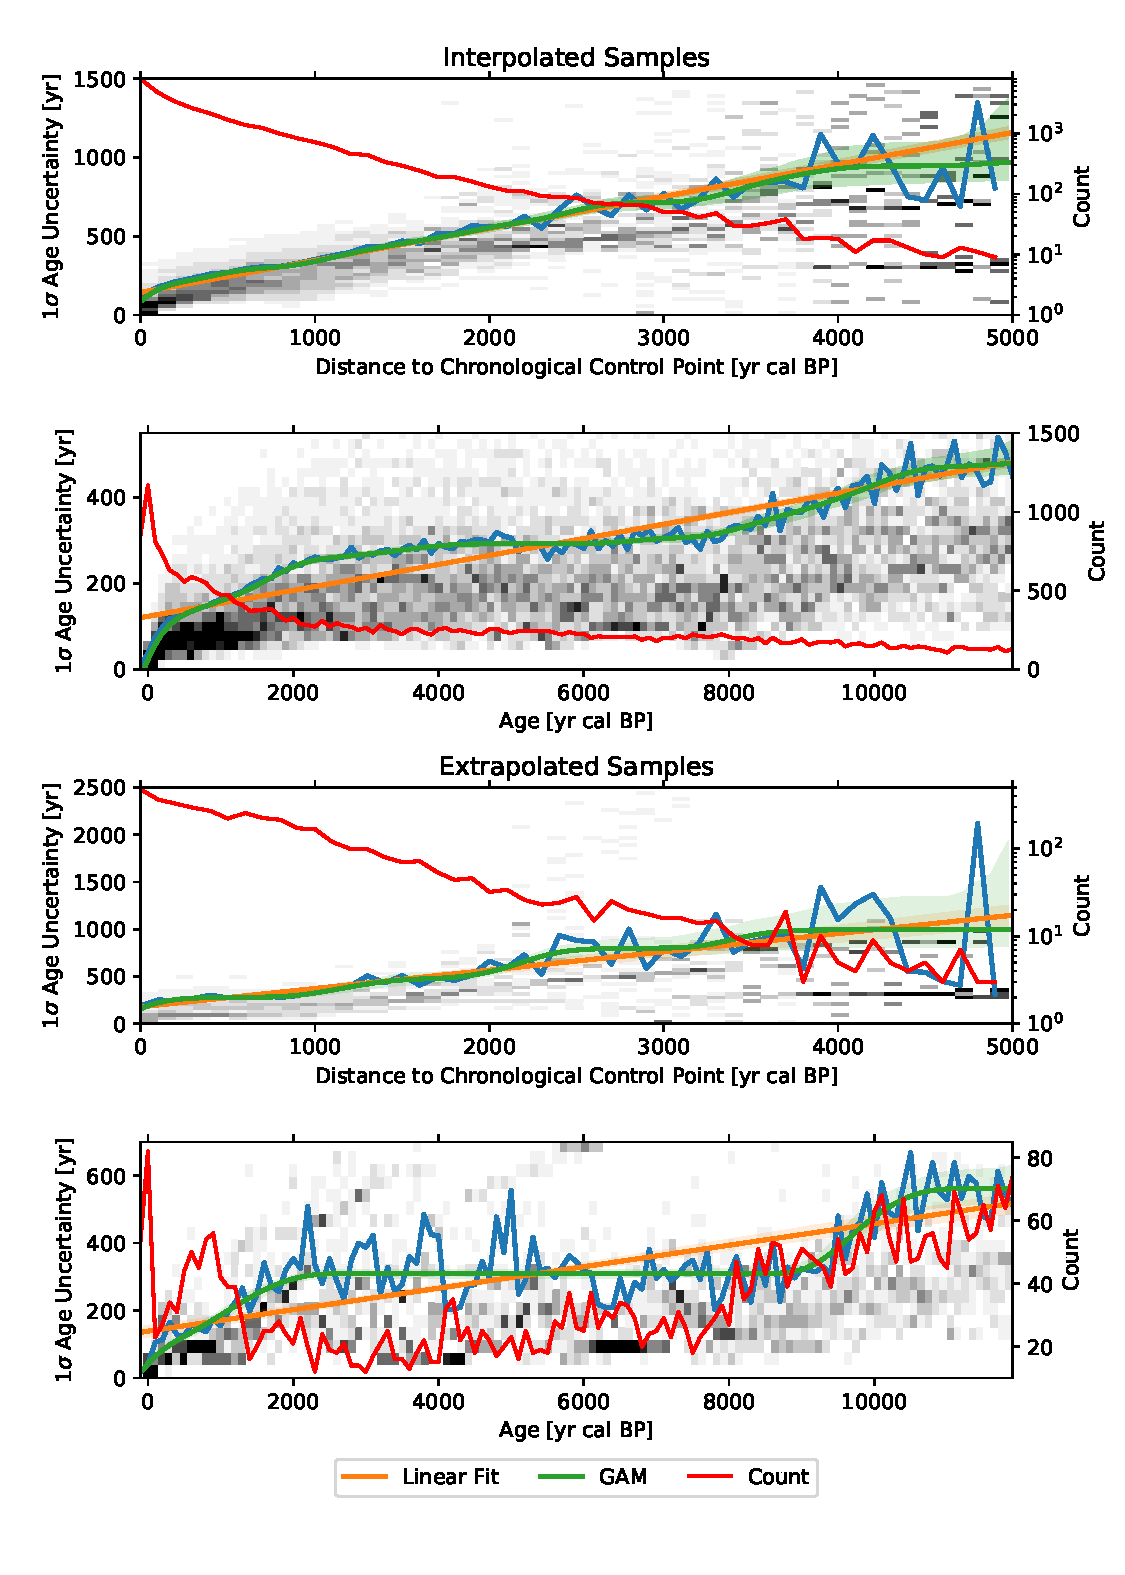
\includegraphics[width=\linewidth]{gridding-figures/univariate-models.pdf}
	\caption[Univariate age uncertainty models]{Univariate regression plots of (first and third) distance to chronological points, and (second and fourth) age to the one sigma dating uncertainty of the sample. The upper two plots contain only interpolated samples (i.e. samples that lie between two chronological control points), the lower extrapolated samples. Blue lines show the mean age uncertainty for the given distance (age). Orange and green lines show the linear and \gls{gam} fits of distance (age) to age uncertainty, and red lines show the number of samples for a given distance (age). The grayscale plot in the background shows a two-dimensional histogram (density plot) to illustrate the underlying data of the fits. For the purpose of a better visualization, each vertical bin of this histogram has been normalized to one. Means, counts and histogram are all based on 100 year bins in distance (age). The fits are estimated based on the unbinned data, the source data are all Neotoma datasets with BACON-based age-depth models. Note the logarithmic scale of the right count axis on the first and third plot.}
	\label{fig:gridding-univariate-age-unc}
\end{figure}

\begin{figure}
	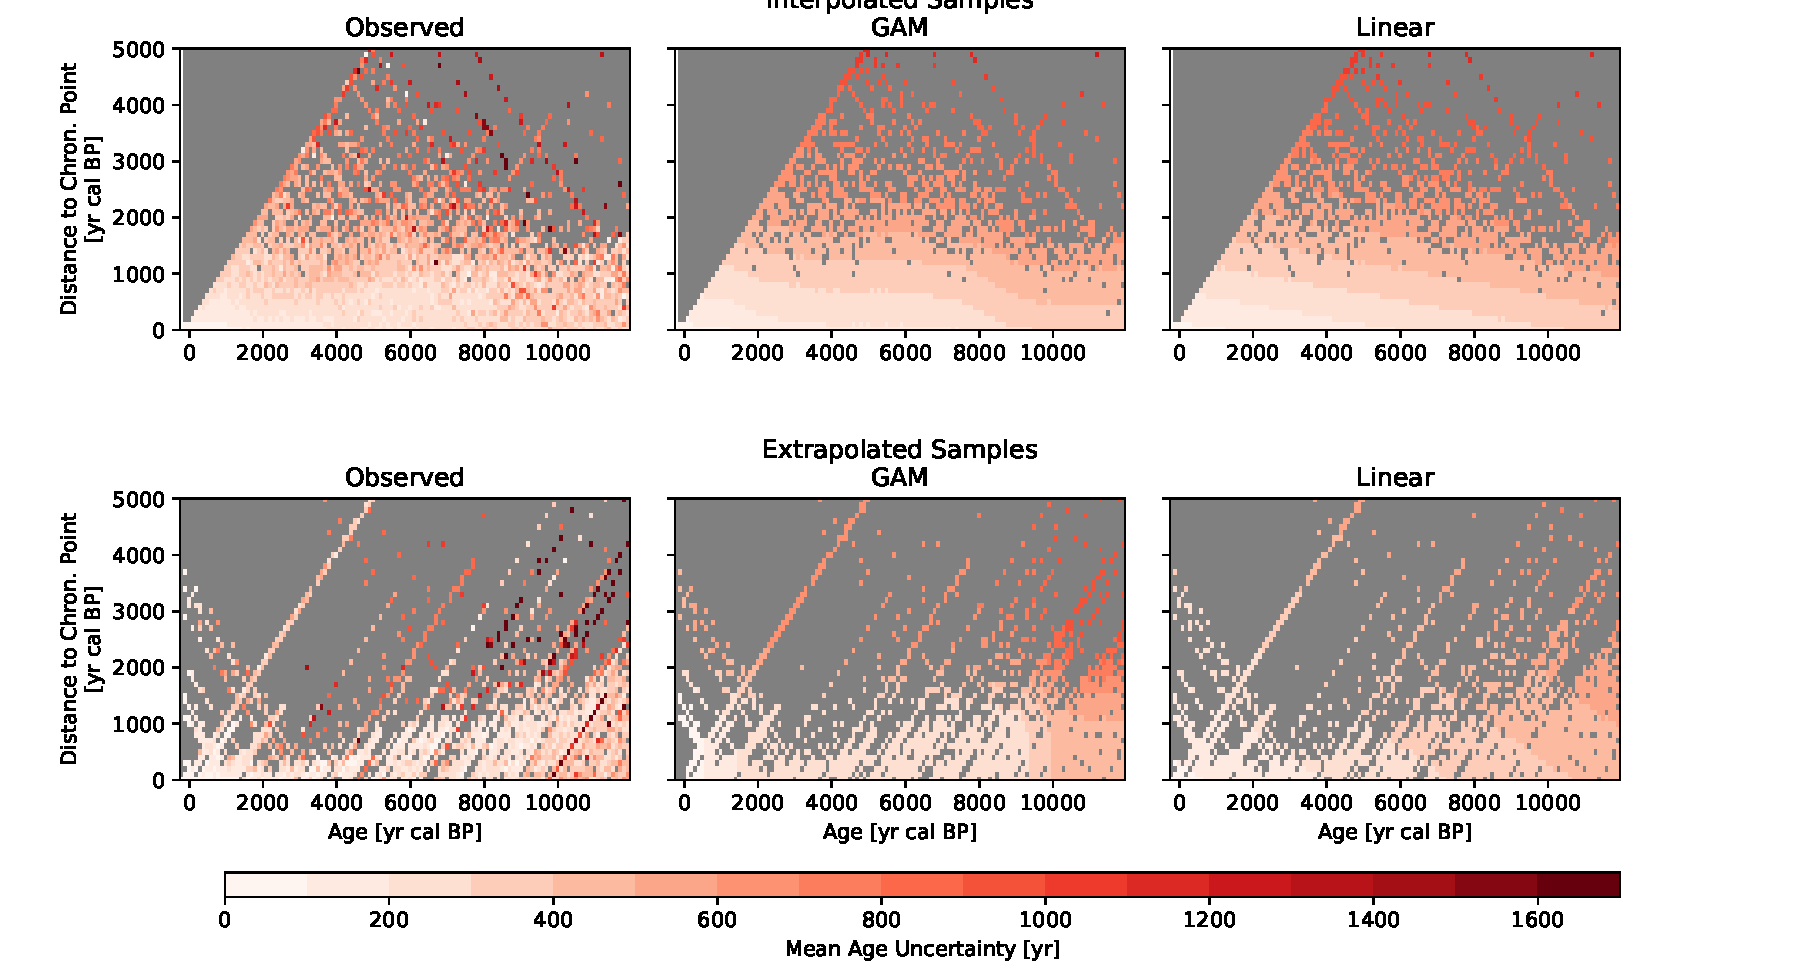
\includegraphics[width=\linewidth]{gridding-figures/bivariate-models.pdf}
	\caption[Univariate age uncertainty models]{Bivariate models of age uncertainty. The top row shows interpolated samples (i.e. samples that lie between two chronological control points), the bottom row extrapolated samples. Plots in the left column show the observed data (samples of the Neotoma database with BACON-based age-depth models), central and right columns show the simulations of bivariate linear \glspl{gam} or bivariate linear regression models respectively. y-axes are the distance to the closest chronological control point, x-axes are the age of the sample, both binned into 100-years intervals. The color coding of each 100 by 100 years grid cell is based on the mean age uncertainty of all samples within this cell.}
	\label{fig:gridding-bivariate-age-unc}
\end{figure}

\section{Method}  \label{sec:gridding-method}
With the intrinsic methodological uncertainties of climate and dating in mind, we present a new ensemble-based approach on gridding the reconstructions from the individual sites. Each ensemble member is generated with an randomized sample ages and climate, derived from the corresponding uncertainty measures (see previous sections \ref{sec:gridding-mat} and \ref{sec:gridding-ageunc}), with additional constrains arising from the integrity of the individual dataset (sediment core). We explain these in more details in sections \ref{sec:gridding-age-sampling} and \ref{sec:gridding-temperature-sampling}. The final gridding step for each ensemble member is based on a modified setup of \cite{MauriDavisCollinsEtAl2015}, but can also be extended with other interpolation algorithms, as described in section \ref{sec:gridding-gridding}). We implemented the method as the python package \textit{pyleogrid} that efficiently scales to large datasets and ensemble sizes, and shortly describe it in section \ref{sec:gridding-package}.

\subsection{Constrained age sampling}  \label{sec:gridding-age-sampling}

\begin{figure}
	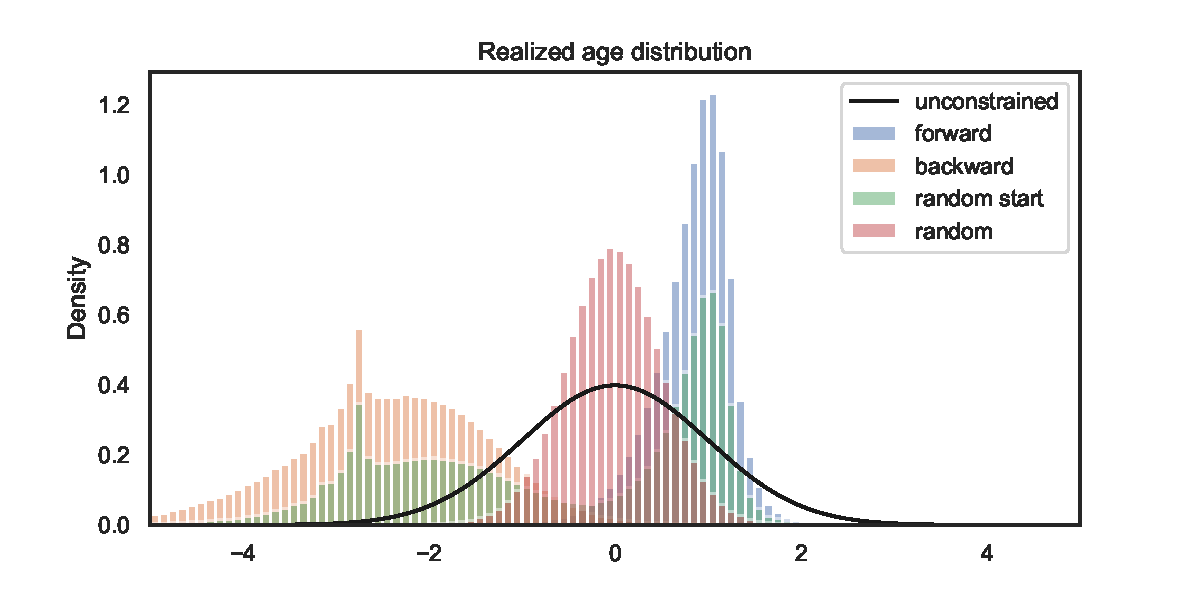
\includegraphics[width=\linewidth]{gridding-figures/age-sampling-methods-realized.pdf}
	\caption[Scaled histograms of age sampling methods]{Histograms of standardized age sampling methods for the site in section \ref{sec:gridding-site} with and ensemble size of 10'000. Every sampled age has been centered at the reported age or the corresponding sample and scaled by its age uncertainty. The black line shows the unconstrained distribution (a standard normal with a standard deviation of 1), the other histograms show the realized distributions for each of the age sampling methods (section \ref{sec:gridding-age-sampling}).}
	\label{fig:gridding-age-sampling-methods}
\end{figure}

Every dataset has an intrinsic monotonicity constrain that the sample deeper down the core has an older age. An inversion of this constrain is very rare and is usually visible in the stratigraphy of the core, such that affected samples are ruled-out before. As such, a classic unconstrained sampling of ages\footnote{\label{foot:unconstrained-note}We call it the unconstrained distribution for convenience, but keeping in mind that every sampled age has to be older than -70 yr cal BP.} using a normal distribution centered at reported sample age and a scale corresponding to the estimated age uncertainty (section \ref{sec:gridding-ageunc}) violates this constrain. Samples are inverted in such a case when their uncertainty intervals overlap and as such the individual ensemble member would not maintain the integrity of the individual core. We illustrate an example for such a core in section \ref{sec:gridding-site}.

\textit{pyleogrid} therefore implements different variants of this constrain. 

\subsubsection{The intuitive approach}
The most intuitive approach is to randomly draw a sample age and constrain the age of the neighboring sample with it. This can be done in a \textit{forward} manner, such that every older sample has to be older than the previous younger sample, or in a backward manner, i.e. the younger sample has to be younger than the neighboring older sample. We will show in the paragraphs below that this method is not working, nevertheless we mention it here because of the intuitivity of the approach and because the reason for the failure is non-trivial.

As such, we demonstrate three different algorithms:

\begin{description}
	\item[forward] Starting with an unconstrained age distribution for the youngest sample in the core, every consecutive sample has to be older than the previous (i.e. the method works forward in age, but backward in time
	\item[backward] Starting with an unconstrained age distribution for the oldest sample in the core, every consecutive sample has to be younger than the previous (i.e. the method works backward in age, but forward in time)
	\item[random start] Starting with an unconstrained age distribution of a random sample in the core, we apply the \textit{backward} algorithm for younger and \textit{forward} algorithm for younger samples.
\end{description}

As such, \textit{forward} and \textit{backward} algorithms always start with an unconstrained age distribution of the youngest (oldest) sample for every ensemble member. Within the \textit{random start} algorithm, every sample gets the chance to start with an unconstrained age distribution, because the starting point is random for every ensemble member. The constrained age distributions for the consecutive samples are implemented as truncated normal distributions.

The resulting age distributions from the three algorithms are shown in figure \ref{fig:gridding-age-sampling-methods}, together with another method, that is described later in this section. The figure shows the sampled age distributions by the various above-mentioned sampling methods for the site described in section \ref{sec:gridding-site}. To make these age distributions comparable, we transformed them to a standard normal distribution (visualized as the unconstrained distribution in figure \ref{fig:gridding-age-sampling-methods}) prior to visualization, by subtracting the reported age and dividing by the estimated age uncertainty of the corresponding sample. It is obvious from this figure that all of the above-mentioned algorithms produce an artificial bias to the age distribution. The \textit{forward} approach pushes the samples to the upper tail of the distribution, the \textit{backward} approach pushes everything to the lower tail. The \textit{random start} method produces a bimodal distribution with peaks at the upper and lower tail.

This is also shown with three exemplary samples from the site in the supplementary figure \ref{fig:gridding-age-example-distributions}. The forward method works well for the young sample but pushes all older samples to the upper tail of their distribution, The backward method does the opposite and the random sort method creates a bimodal distribution for the sample in the center of the core, and backward behaves like the forward (backward) algorithm at the older (younger) part of the core.

We explain this initially unexpected results with the overlapping age uncertainties in the core. The site that we describe here has 110 samples. As such, the probability that one sample draws a random age at the lower or upper tail of the distribution is very high. Now, most of the dating uncertainty intervals overlap and this forces all the consecutive samples to the tail of their age distributions. Another problem, that is not shown here, arises from the differing sizes of the age uncertainties which highly depends on the distance to the chronological control point (see section \ref{sec:gridding-ageunc}). This can also lead to unsatisfiable requirements, if one sample is close to a control point (and as such has a lower age uncertainty) and the previous sample has been pushed far outside of the 95\% confidence interval.


\subsubsection{The random sorting approach}

\begin{figure}
	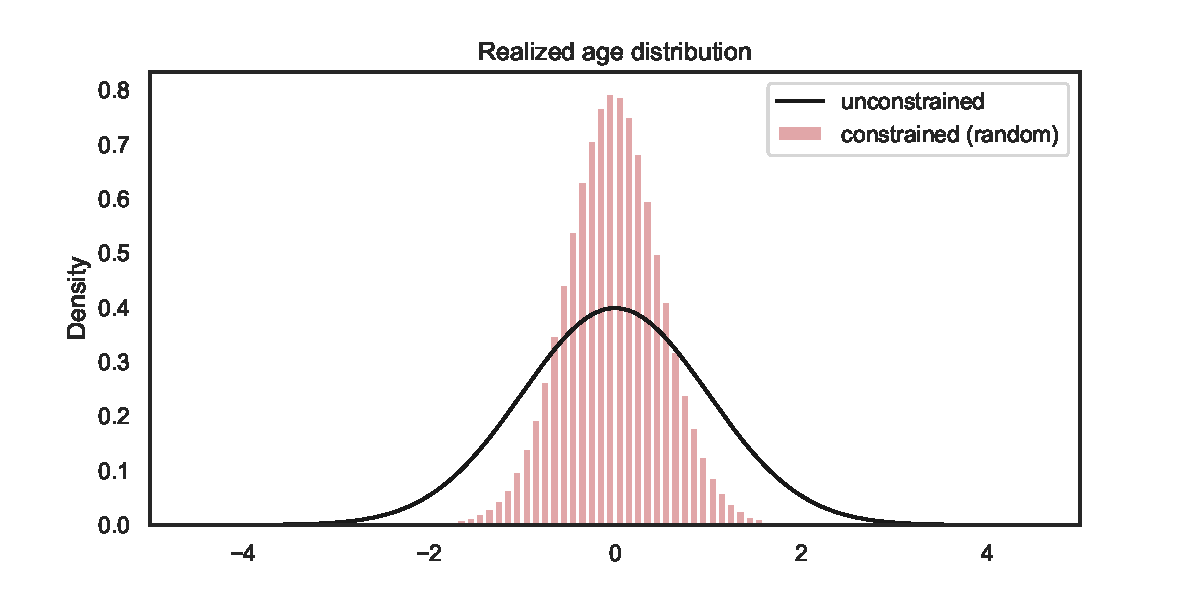
\includegraphics[width=\linewidth]{gridding-figures/full-realized-age-distribution.pdf}
	\caption[Realized age distribution for the entire dataset]{Realized age distribution for the entire dataset (section \ref{sec:gridding-polnet}) with the \textit{random} method (section \ref{sec:gridding-age-sampling}). The individual sample distributions have been centered and scaled as in figure \ref{fig:gridding-age-sampling-methods}.}
	\label{fig:gridding-full-age-distribution}
\end{figure}

These strong biases of the intuitive approach led to another method, that we also show in red in figure \ref{fig:gridding-age-sampling-methods} and supplementary figure \ref{fig:gridding-age-example-distributions}, the \textit{random} method. This method consists of two steps: in the first step we draw random age for each sample based on its unconstrained distribution\textsuperscript{\ref{foot:unconstrained-note}}. In the second step, we order these random ages while maintaining the order of samples in each dataset. As such, we assign an age to each sample that is not necessarily drawn from its own distribution, but rather from the one of a neighboring sample. When samples overlap, this then truncates the tails of realized distribution and effectively decreases the reported age uncertainty, as can be seen in the figures \ref{fig:gridding-age-sampling-methods}, \ref{fig:gridding-age-example-distributions} and for the full dataset in figure \ref{fig:gridding-full-age-distribution}. This approach violates the common approach that each sample has a unique confidence interval that it needs to explore and as such might introduce some hidden biases in the sampled distributions. Nevertheless, the algorithm is very fast and much closer to the  desired joint distribution, than the previous \textit{intuitive} approach.


\subsubsection{The Gibbs sampling approach}
The biases of the above-mentioned algorithms led to the development of a \gls{mcmc} sampling algorithm. A standard \gls{mcmc} approach, is to draw a set of random ages for all unconstrained sample distributions in a core at once, until this set of ages satisfies the monotonicity criterion. This is described with the following pseudo-code:

\begin{algorithm}
	\renewcommand{\algorithmicensure}{\textbf{Output:}}
	\caption[Classic MCMC approach]{Classic \gls{mcmc} approach}
	\label{a:gridding-mcmc}
	\begin{algorithmic}[1]
		\FOR{$dataset$ in $datasets$}
		\STATE Set $i = 0$
		\STATE Set $\vec{\mu}$ as vector reported ages in $dataset$
		\STATE Set $\vec{\sigma}$ as estimated age uncertainties		
		\STATE Set $\vec{ages}$ to be of length $\vec{\mu}$
		\WHILE{$i < 1$ \OR \NOT $is\_monotonic(\vec{ages})$}
		\STATE $\vec{ages} = \mathcal{N}(\vec{\mu}, \vec{\sigma}^2)$
		\STATE Set $i = i + 1$
		\ENDWHILE
		\ENDFOR
	\end{algorithmic}
\end{algorithm}

This standard approach however did not find a monotonic solution within ten million iterations for a high-resolution site such as it has been presented in the previous section. Therefore we decided to implement a Gibbs sampler, an algorithm that is commonly used in Bayesian inference. \todo[inline]{Describe Gibbs sampler}

\subsection{Temperature sampling}  \label{sec:gridding-temperature-sampling}
\begin{itemize}
	\item Sampling of analogue climates weighted by squared chord distance
	\item Can also use different methods (WAPLS, etc.)
	\item Random starting point
	\item Mask analogues that have a temperature distance more than 5°C??? From the previous/earlier sample – test this
\end{itemize}
As mentioned in section \ref{sec:gridding-mat}, our method alters the standard \gls{mat} approach such that it does not use the weighted average, as it is commonly estimated, but \todo{continue}

\subsection{Gridding}  \label{sec:gridding-gridding}
\begin{itemize}
	\item 3D of climate (not anomaly)
	\item Distance in time through weighting
	\item Paleo-Elevation (ICE-6G)
	\item Can use any other method than tps
\end{itemize}

\subsection{Implementation}  \label{sec:gridding-package}

\section{Results}  \label{sec:gridding-results}

\subsection{Site-based realized climate reconstruction: a use-case} \label{sec:gridding-site}
\todo[inline]{Reconstruction of entity 11390}

\section{Discussion}  \label{sec:gridding-discussion}

\begin{itemize}
	\item Maps of reconstruction
	\begin{itemize}
		\item How high are the uncertainties
	\end{itemize}
	\item Questions: 
	\begin{itemize}
		\item How does the uncertainty evolve with distance to the samples
		\begin{itemize}
			\item At map boundaries
			\item In gaps within the data
		\end{itemize}
	\end{itemize}
	\item How consistent is the interpolation uncertainty (from Tps) within the ensemble?
\end{itemize}


\section{Conclusions}  \label{sec:gridding-conclusions}

\clearpage

\begin{subappendices}
	\section*{Supplementary material}
	
	\section{Estimated age uncertainties}  \label{sec:gridding-suppl-age-uncertainties}	
		\begin{figure}[!h]
			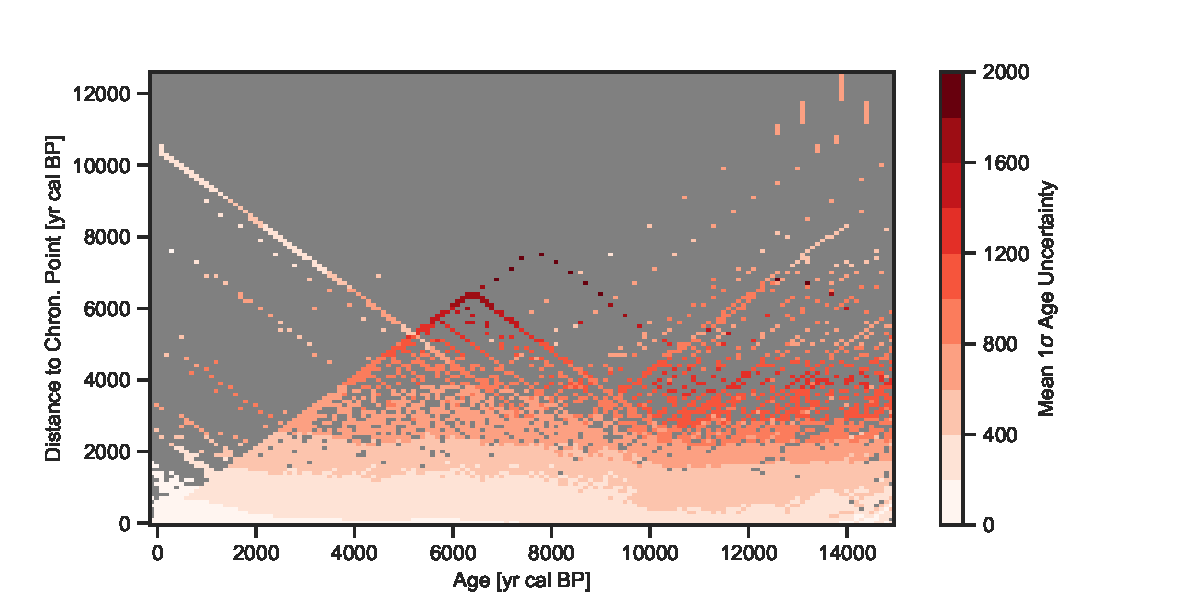
\includegraphics[width=\linewidth]{gridding-figures/realized-age-uncertainties.pdf}
			\caption[Estimated age uncertainties]{Estimated age uncertainties for the Eurasian dataset from section \ref{sec:gridding-polnet} with the same formatting as in figure \ref{fig:gridding-bivariate-age-unc}.}
			\label{fig:gridding-age-uncertainties}
		\end{figure}
	
	\clearpage

	\section{Example of generated age distributions} \label{sec:gridding-suppl-age-example-distributions}
		\begin{figure}[!h]
			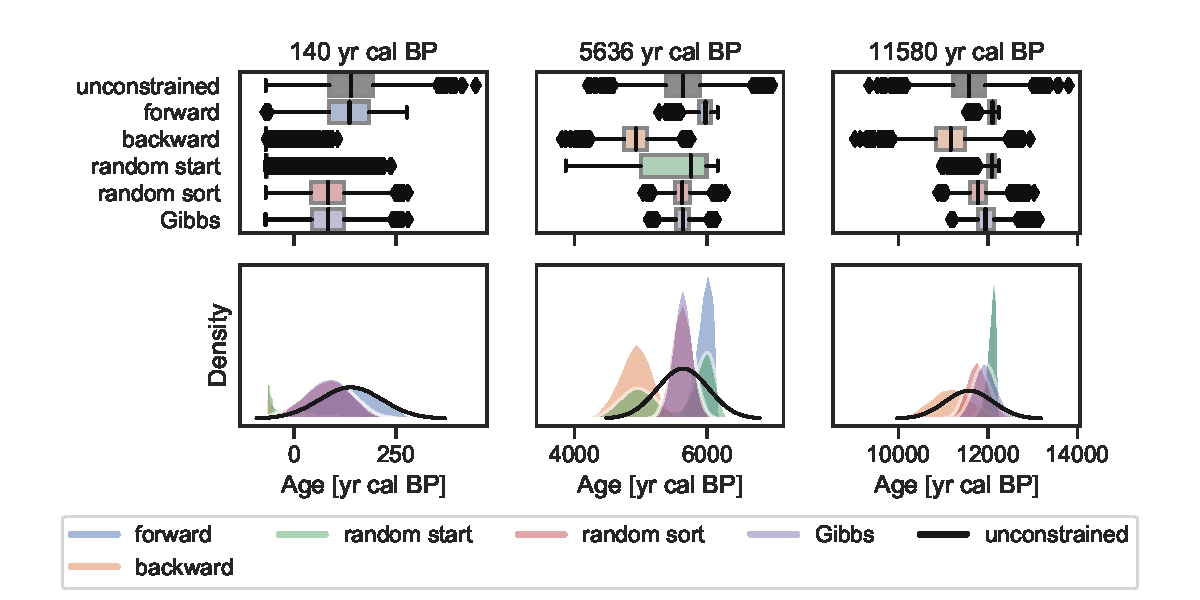
\includegraphics[width=\linewidth]{gridding-figures/age-sampling-methods-use-case.pdf}
			\caption[Example of sampled distribution]{Example of three samples from the site in section \ref{sec:gridding-site} and their realized distributions. Sampling algorithms are explained in section \ref{sec:gridding-age-sampling}. Top plots show the box plots of the realized distribution that are visualized with a kernel density estimate in the lower row.}
			\label{fig:gridding-age-example-distributions}
		\end{figure}

\end{subappendices}

\printbibliography[heading=subbibintoc]

\end{refsection}